\chapter{\label{chap:related-work}Trabalhos Relacionados}

\begin{mdframed}[backgroundcolor=green!20]
\begin{itemize}
	\item
		Breve descrição deste capítulo
    \item
        Encontrar trabalho relacionado sobre Behavior Trees
\end{itemize}
\end{mdframed}


%----------
\section{Playing Atari with Deep Reinforcement Learning}
O artigo apresenta um modelo de \textit{deep learning} capaz de aprender
políticas de controle para sete jogos do \textit{console} Atari 2600, criando
uma inteligência artificial capaz de jogar eficientemente todos os jogos,
inclusive superando jogadores humanos em alguns
deles\cite{DBLP:journals/corr/MnihKSGAWR13}. O modelo utiliza aprendizado por
reforço e uma rede neural convolucional treinada com uma variante de
\textit{Q-learning} para criar o agente.

Para criar estas políticas de controle, os autores utilizaram uma plataforma de
testes de inteligência artificial chamada \textit{Arcade Learning Environment}.
A cada passo de execução, o agente interage com o emulador, recebendo
informações do estado do jogo e enviando os comandos que deseja executar. As
informações recebidas eram um vetor dos \textit{pixels} apresentados na tela, o
conjunto de de ações possíveis para o jogo em questão e um valor de recompensa
quando a pontuação do jogo era alterada.

Como as informações do estado do jogo eram altamente dimensionais -- 33600
\textit{pixels} de informação visual --, foi necessário realizar um
pré-processamento para reduzir a dimensionalidade do estado do jogo -- reduzindo
para 7600 \textit{pixels}. Mesmo com esta redução, a quantidade de informações
recebidas ainda era consideravelmente grande. Por isto, a utilização de
\textit{deep learning} e redes neurais convolucionais provou ser uma excelente
-- e necessária -- escolha para realizar o treinamento do agente. Contudo, o
treinamento do agente utilizando esta técnica é extremamente demorado.

Como a dimensionalidade do estado do jogo fornecido pela ferramenta
\textit{SpelunkBots} não é tão grande quanto a do trabalho em questão, optamos
por não fazer uso de \textit{deep learning}, mesmo que a técnica também seja
muito promissora.


%----------
\section{MarI/O}
Em junho de 2015, o canal do \textit{YouTube}
SethBling\footnote{https://www.youtube.com/user/sethbling/about} -- conhecido
por publicar vídeos de modificações de jogos como Mario e Minecraft -- divulgou
o vídeo \textit{MarI/O - Machine Learning for Video
Games}\footnote{https://www.youtube.com/watch?v=qv6UVOQ0F44}, que mostra um
jogador muito habilidoso completando o nível \textit{Donut Plains 1} de
\textit{Super Mario World}. É explicado, então, que o jogador em questão não é
humano, mas sim um programa de computador. Utilizando um emulador de
\textit{consoles} chamado
\textit{BizHawk}\footnote{http://tasvideos.org/BizHawk.html}, a linguagem de
programação \textit{Lua} e uma técnica de inteligência artificial chamada
\textit{\textbf{N.E.A.T}} (\textit{NeuroEvolution of Augmenting Topologies})
\cite{stanley:ec02} -- explicada detalhadamente no capítulo \ref{chap:neat} --,
o autor programou um \textit{bot} capaz de aprender como jogar o nível em
questão do início ao fim com sucesso. Como é explicado no vídeo, inicialmente o
\textit{bot} não conhecia absolutamente nada sobre como jogar \textit{Super
Mario World}. Contudo, através de várias simulações, adquiriu o conhecimento
necessário para superar todos os obstáculos presentes no nível.

\begin{figure}[htb!]
\centering
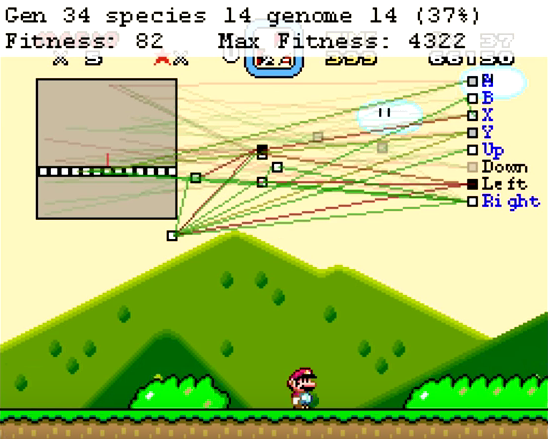
\includegraphics[width=.65\textwidth]{fig/mar-io-example.png}
\caption{\label{fig:mar-io-example}Exemplo da visão do jogo \textit{Super
Mario World} através do projeto \textit{MarI/O}, mostrando elementos de
controle usados pelo NEAT, como a rede neural, as possíveis ações, as
gerações, as espécies, os genomas, entre outros.}
\end{figure}

Depois do sucesso no nível \textit{Donut Plains 1}, o autor realizou mais
experimentos da aplicação da técnica
\textit{NEAT}\footnote{https://www.youtube.com/watch?v=iakFfOmanJU}
\footnote{https://www.youtube.com/watch?v=S9Y\_I9vY8Qw}. Inicialmente, testou em
dois outros níveis de \textit{Super Mario World}. Em \textit{Donut Plains 4}, o
processo de aprendizagem foi complicado, pois para obter progresso no nível era
necessário que aprendesse a interagir com certos elementos do mapa, e o autor
decidiu abortar o processo de aprendizagem. Já em \textit{Yoshi's Island 1},
obteve sucesso e foi capaz de concluir o nível. Com os testes finalizados, o
autor decidiu aplicar a técnica em outros dois jogos da franquia \textit{Mario}.
Em \textit{Super Mario Bros}, o \textit{bot} concluiu o primeiro nível e,
surpreendentemente, foi capaz de descobrir um \textit{glitch} no jogo que o
permitia passar por um segmento do segundo nível com maior rapidez. Em
\textit{Super Mario Kart}, depois de receber treinamento, o \textit{bot} foi
capaz de terminar uma corrida no nível \textit{Mario Circuit 1} em primeiro
lugar contra outros jogadores controlados pelo computador -- na dificuldade mais
fácil do jogo.

O \textit{MarI/O} é especialmente interessante e relevante porque tem um
objetivo muito similar ao deste trabalho: criar uma inteligência artificial
capaz de jogar uma partida de um jogo. Contudo, nos jogos escolhidos por
SethBling, os níveis são sempre os mesmos, o que torna mais fácil medir o
desempenho de um \textit{bot}, pois a disposição do nível é sempre igual e o
objetivo final sempre se encontra no mesmo lugar. Este não é o caso em
\textit{Spelunky}, onde os níveis são gerados proceduralmente. Além disso, os
níveis de \textit{Super Mario World} e \textit{Super Mario Bros.} são
essencialmente horizontais, e movimentar o personagem para a direita quase
sempre garante alguma forma de progresso. Isto facilita ainda mais o processo de
treinamento dos \textit{bots}. Em \textit{Spelunky} não é possível saber de
antemão onde se encontra a saída do nível e o movimento horizontal não garante o
progresso, visto que os níveis não são essencialmente horizontais. Estes fatores
influenciam na dificuldade de realizar o treinamento dos \textit{bots}.
